% spellchecker:disable
\documentclass[pdftex,
	chapterprefix,
	headsepline,
	footsepline,
	% colordvi,
	11pt,
	a4paper,
	parskip=half,
	% enabledeprecatedfontcommands,
	final,
	appendixprefix,
	bibliography=totoc]{scrbook}

% define a new if command to distinguish between PDF and DVI output
\usepackage{ifpdf}
\ifx\pdfoutput\undefined
\pdffalse %not PDFLaTeX
\else
\pdfoutput=1
\pdftrue
\fi

% language support (hyphenation etc)
% this sets the main language of the paper to english
% if you wish to compose it in german, switch the options around
\usepackage[german,english]{babel}

% for prettier tables
\usepackage{booktabs}

% support for latin1 characters. That means you can enter umlauts directly
% no need for "a "u "o "s anymore
\usepackage[utf8]{inputenc}
\usepackage{textcomp}

% provides the \url{} command to pretty print urls
\usepackage{url}

% allows to \includegraphics
\usepackage{graphicx}
\usepackage{svg}

% defines some standard colornames like "black" etc.
\usepackage{color}

% allows to color tablecells
\usepackage{colortbl}

% provides an easier interface to if-then-else constructs in custom macros
\usepackage{ifthen}

% allows tables to break over pages.
\usepackage{supertabular}

% allows to have different kinds paper orientations in the same pdf-documnent
\usepackage{pdflscape}

% allows to specify absolute texpos for textboxes. This is generally only important for the titlepage
\usepackage[absolute]{textpos}

% % allows to enumerate different figures with a) b) in the same figure-environment.
\usepackage{subfigure}

\usepackage{caption}
\DeclareCaptionLabelFormat{cont}{#1~#2\alph{ContinuedFloat}}
\captionsetup[ContinuedFloat]{labelformat=cont}

% math
\usepackage{amsmath}

% allows inserting source code
\usepackage{listings}
\usepackage{scrhack} % fixes lst incompatibility
\lstset{
% numbers=left,              % Location of line numbers
	numberstyle=\tiny,          % Style of line numbers
	numbersep=5pt,              % Margin between line numbers and text
	tabsize=4,                  % Size of tabs
	extendedchars=true,
	breaklines=true,            % Lines will be wrapped
	showspaces=false,
	showtabs=false,
	showstringspaces=false
}

% More fancy syntax highlighting: https://texdoc.net/texmf-dist/doc/latex/minted/minted.pdf
% careful, this has additional external dependencies
%\usepackage[newfloat]{minted}
% configure source code highlighting; edit this to your liking
% style=bw will save you some money on color pages, but may be harder to read
%\setminted{
%	style=stata-light,
%	frame=leftline,
%	breaklines=true,
%	numbers=left,
%	tabsize=4}

% allows usage of BibLaTeX for bibliography; needs the Biber tool!
\usepackage[
backend=biber,
sorting=anyt
]{biblatex}
\usepackage{csquotes}
% point this to your bibliography file
\addbibresource{bib/references.bib}

% finetune the gaps between figure and text in the subfigure environment (basically close the gap as much as possible)
\renewcommand{\subfigtopskip}{0pt}
\renewcommand{\subfigbottomskip}{0pt}

% some color definitions for the pdf statements below
\definecolor{mygrey}{rgb}{0.45,0.45,0.45}
\definecolor{mydarkgrey}{rgb}{0.2,0.2,0.2}
\definecolor{red}{rgb}{1.0,0.33,0.33}
\definecolor{orange}{rgb}{1.00,0.73,0.33}
\definecolor{yellow}{rgb}{0.95,0.92,0.}
\definecolor{lightgreen}{rgb}{0.3,0.95,0.46}
\definecolor{titleblue}{rgb}{0.03,0.10,0.46}

\ifpdf
% For screen viewing it is nice to have references marked in a slightly different
% color than the rest of the text. Since they will be hyperlinks to the
% referenced objects.
\usepackage[pdftex,
	pdftitle={Fancy thesis template},
	% colorlinks,
	% linkcolor={black},
	% citecolor={black},
	urlcolor={black},
	plainpages={false},
	bookmarksnumbered={true},
	pdfauthor={Vorname Nachname},
	pdfsubject={},
	pdfkeywords={},
	pdfstartview={FitBH}]{hyperref}

\pdfcompresslevel=9
\fi

% some configuration for the amount of text on a single page
\usepackage{typearea}
\areaset[1.5cm]{418pt}{658pt}
\setlength{\headheight}{37pt}

% enter author and title for the titlepage.
\author{}
\title{}

% To avoid nasty mistakes like having comments directly in the textflow
% the following \todo macro was defined. With that you can enter
% \todo{What I still have to do here}
% inside of your text and a marker will appear at the page's margin with the
% text "What I still have to do here".
% The first line activates this feature. If you comment it out and uncomment
% the second line below there will be no error messages and no todos will be shown
% anymore. So - even if you have forgotten to delete one of them - they will not appear
% in the final printout.
\newcommand{\todo}[1]{\marginpar{\textcolor{red}{TODO:} #1}}

% We recommend to split your document into several files. Usually one for every chapter is a
% good idea. If you follow this guideline (how to assemble these files in a single document
% see two paragraphs below) you will be able to single out chapters via the \includeonly{}
% command. Using this mechanism page numbering and references of the full run before will be
% preserved. This also nice, if your latex run tends to get slow and you need to fine tune
% some formatting in one chapter - just include that one. The rest (or at least the ones before
% the one currently under construction) will remain untouched. This means a boost in compilation time.
%\includeonly{content/chapter2}

\begin{document}

% the next two lines influence the detailedness of the table of contents
% and to what structure depth numbers are written before sections/subsections/paragraphs
% You should not touch this
\setcounter{tocdepth}{2}
\setcounter{secnumdepth}{3}

\frontmatter

% here the titlepage is included. Look into the file "frontpage.tex" to
% adapt it to your needs (name, title etc.)
% spellchecker:disable
\begin{titlepage}
\selectlanguage{german}
\vspace*{-1cm}
\newlength{\links}
\setlength{\links}{0.9cm}
\setlength{\TPHorizModule}{1cm}
\setlength{\TPVertModule}{1cm}
\textblockorigin{0pt}{0pt}

\sffamily
\LARGE

\begin{textblock}{16.5}(2.8,2.6)
 \hspace*{-0.25cm} \textbf{UNIVERSITÄT DUISBURG-ESSEN} \\
 \hspace*{-1.15cm} \rule{5mm}{5mm} \hspace*{0.05cm} FAKULTÄT FÜR INGENIEURWISSENSCHAFTEN\\
 \large{}ABTEILUNG INFORMATIK UND ANGEWANDTE KOGNITIONSWISSENSCHAFT\\
\end{textblock}


%Hier Titel, Name, und Matrikelnummer eintragen, \\ make a newline
\begin{textblock}{14.5}(3.2,8.5)
  \large
{ \textbf{Bachelorarbeit}} \\[1cm]
{\LARGE \Large\textbf{Fancy thesis template}} \\[1.3cm]
Vorname Nachname\\
Matrikelnummer: 0123456\\
Angewandte Informatik (Bachelor)
\end{textblock}



\begin{textblock}{10}(10.5,17.5)

\includegraphics[scale=1.0]{images/unilogo.pdf}\\
\normalsize
\raggedleft
Fachgebiet Verteilte Systeme, Abteilung Informatik \\
Fakultät für Ingenieurwissenschaften \\
Universität Duisburg-Essen \\[2ex]

\today\\[15ex]
\raggedright
% Supervisors
{\textbf{Erstgutachter:}} Prof. Dr-Ing. Torben Weis \\
{\textbf{Zweitgutachter:}} Hier Zweitgutachter eintragen \\
{\textbf{Zeitraum:}} 1. September 2042 - 1. Januar 2043 \\
\end{textblock}

\end{titlepage}


\selectlanguage{english}

\chapter*{Abstract}
Hidden Markov Modelle sein ein weit verbreitetes Werkzeug für Signalmodellierung. Die Parameter eines HMM werden typischerweise mit dem Baum-Welch Algorithmus trainiert, welcher jedoch nur lokale Optima findet. Der Baum-Welch Algorithmus wurde zu Begin der 1970er Jahre entwickelt und ist somit über 50 Jahre alt. In dieser Zeit wurden viele alternative Trainingsverfahren entwickelt mit dem Ziel eine bessere globale Suchkapazität zu bieten. Einige dieser Algorithmen sind sogenannte Metaheuristiken welche oft den Baum-Welch Algorithmus hybridisieren. Ziel dieser Arbeit ist es zu evaluieren in wie weit solche (hybriden) Metaheuristiken geeignet sind für die Parameter-Estimation eines HMM, wobei wir uns in der Auswertung auf genetische Algorithmen beschränken, welche zu den meißterforschten Metaheuristiken zählen. Zu diesem Zweck wurde ein Framework für das trainieren von HMMs mit genetischen Algorithmen entwickelt, mit welchem drei verschiedene Ansätze untersucht werden. Die Auswertung zeigt, dass genetische Algorithmen nicht geeignet sind für das Trainieren von HMMs und das der Baum-Welch Algorithmus nicht ohne Grund weiterhin der Standard für die Parameter-Estimation ist.

\tableofcontents

%\listoffigures
\mainmatter

% To assemble the whole document
% Please be aware that each file will begin on a new page
% therefore chapters should be put into such a file.
% There cannot be an include statement inside of an "included" file.
% So if you want to further divide your document - use \input inside of
% the included files. \input will not begin on a new page.

% \chapter{Introduction}
Hidden Markov Modelle bietet die möglichkeit komplexe Systeme zu modellieren. Sie wurden im frühen zwanzigsten Jahrhundert durch Andrey Markov eingeführt \cite*{rabiner}. Zunächst war die Forschung an Hidden Markov Modellen primär theoretischer Natur, bis in den späten 1960er bis frühen 1970er Jahren effiziente Methoden für die Parameterestimation durch Leonard E. Baum und seine Kollegen entwickelt wurden. Seit jeher sind Hidden Markov Modelle finden praktische Anwendung in einer Vielzahl an Wissenschaftlichen Disziplinen. Hidden Markov Modelle sind beliebt, da sie unter anderem sehr flexibel und einfach zu implementieren sind \cite*{HmmReview} und mittleerweile aus den Gebieten der Spracherkennung \cite*{ApplicationSpeechRecognition} und Bioinformatik \cite*{ApplicationComputationalBiology} nicht mehr wegzudenken. Eine der prominentesten Anwendungen von Hidden Markov Modellen ist der Google Pagerank Algorithmus, welcher die Relevanz von Website in Relation zu einer Suchanfrage ermittelt \cite*{ApplicationPageRank}.

\subsubsection*{Motivation}
Wie gut ein trainiertes Hidden Markov Model einen Prozess modeliert ist abhängig von der Qualität der Parameter des Modells. Die am häufigsten verwendete Methode für das ermitteln der Parameter ist der Baum-Welch Algorithmus. Dieser ist jedoch anfällig dafür in lokalen Optima stecken zu bleiben. Daher wurden in den letzten Jahren zahlreiche alternative Trainingsverfahren für HMMs entwickelt. Viele davon sind sogenannte Metaheuristiken, stochastische Verfahren die durch natürliche Prozesse wie Evolution inspiriert sind. Trotz dieser großen Auswahl alternativer Trainingsverfahren besteht die predominante Trainingsstrategie weiterhin darin, den Baum-Welch Algorithmus mehrmals auf verschiedene initiale Parametern anzuwenden und das beste resultierende Modell zu wählen. So lautet es zumindestens in der Dokumentation zu \textit{hmmlearn}, einer der beliebtesten HMM python libraries. Es stellt sich also die Frage warum keine der alternativen Trainingsverfahren so großen Anklang wie der Baum-Welch Algorithmus gefunden hat.

\subsubsection*{Struktur}
Ich werde zunächst die Grundlagen auslegen, dazu gehören eine Übersicht zum Aufbau und stochastische Methoden für Hidden Markov Modelle. Danach widmen wir uns allgemeiner dem Gebiet der Optimierung und gehe auf Metaheuristische Algorithmen ein sowie derer Kritik. Danach werden genetische Algorithmen erklärt. Im zweiten Kapitel werden die Konzepte aus den Grundlagen kombiniert und es wird darauf eingegangen wie man Hidden Markov Modelle mit einem genetischen Algorithmus kombinieren kann und worauf man dabei achten sollte. Des Weiteren wird ein Überblick verschafft über die bisher unternommenen metaheuristischen Trainingsansätze für HMMs. Im dritten Kapitel gehe ich auf die Implementation eines Frameworks für genetische Algorithmen und Hidden Markov Modelle ein. Danach werden drei Ausgewählte Ansätze die Hidden Markov Modelle mit einem genetischen Algorithmus trainieren evaluiert. Die Arbeit konkludiert mit einem Fazit über die feasibility von genetischen Algorithmen für das training von HMMs, so wie einer Diskussion über den Zustand des Feldes der Metaheuristischen Optimierung und gibt einen Ausblick über zukünftige Forschung. 

% \chapter{Related Work}\label{ch:related_work}

This chapter presents the basis on which the system and later evaluation are built.
It usually contains short descriptions of previous research papers
and puts them into the context of the thesis.

\section{Code Listings}

If there is some interesting code you would like to show
in order to ease the understanding of the text,
you can just include it using the \verb+lstlisting+ environment.
Have a look at the source of this page to see how this is included:

\begin{lstlisting}[language=Go]
x := from(42);
\end{lstlisting}

You could also put the code into an external file
and include it in this document using the \verb+lstinputlisting+ command:

\lstinputlisting[language=Go,numbers=left]{listings/example.go}

Be careful not to include large files as it hampers readability.
If there is a short excerpt from a large file you would like to show,
you can also extract an explicit range of lines from it without the need to modify the source file.
This next listing only shows the conditional from the previous code:

\lstinputlisting[language=Go,numbers=left,firstline=2,lastline=5,firstnumber=2]{listings/example.go}

To use more advanced syntax highlighting
have a look at the available options of the \emph{listings} package
or use the \emph{minted} package\footnote{\url{https://texdoc.net/texmf-dist/doc/latex/minted/minted.pdf}},
which has more extensive language support and additional themes.
Both can be configured in the main file.
 % input does not start a new page
\section{Math}

In case you need to include some math,
the \emph{amsmath} package\footnote{\url{https://texdoc.net/texmf-dist/doc/latex/amsmath/amsmath.pdf}} is already included in this document.

To properly display some short formula like \( e^{i \pi} = -1\),
you can use the \verb+\( \)+ inline command.
For larger formulas, the \verb+math+ environment is more appropriate.
If you need to reference the formula multiple times,
e.g. in case it is used in theorems,
you should use the \verb+equation+ environment:

\begin{equation}
	\vec\nabla\times\vec{B}= \mu_0\vec{j}+\mu_0\varepsilon_0\frac{\partial\vec{E}}{\partial t}
	\label{func}
\end{equation}

To reference it as~\ref{func} using the \verb+\ref{}+ command,
remember to use a \verb+\label{}+.

\section{Miscellaneous}

You can use the \verb+\todo{}+ command to put obvious reminders on the side of the document.\todo{like this!}


% \chapter{Evaluation}\label{ch:eval}

The evaluation usually consists of three main steps:
first it defines the goals intended to be achieved by the software in detail;
next is a description of the methodology
used to measure the satisfaction of the software in relation to these goals;
finally, the measurements are depicted and assessed.


% \chapter{Conclusion}

The conclusion quickly summarizes the results of the paper
in relation to the previously defined goals and hypotheses.
It usually also includes some information on next steps and further research
that might be required or possible on the presented subject.


\chapter{Trainieren von HMMs mit einem GA}\label{ch:gahmm}


\section{Konstruktion eines GAHMM}

In diesem Kapitel werde ich beschreiben wie man einen Genetischen Algorithmus 
für Hidden Markov Modelle erstellen kann und dann auf die in meiner Arbeit verwendeten 
konkreten Implementationen der genetischen Operatoren eingehen.



\subsection*{Representation}
Ähnlich wie in den Papers [hier papers einfügen] 
Ist die Chromosonale Representation eines HMMs ein Vektor welcher 
die Reihen aller Matrizen hintereinander enthält.

Um die Struktur von nicht ergodischen Hidden Markov Modellen im Mutations-schritt nicht zu Verändern 
muss man die Gene Welche Startwahrscheinlichkeiten und Transitionswahrscheinlichkeiten
beschreiben von der Mutation ausschließen oder man kann eine Maske definieren
welche eine Mutation Gene welche initial 0 oder 1 sind verhindert.


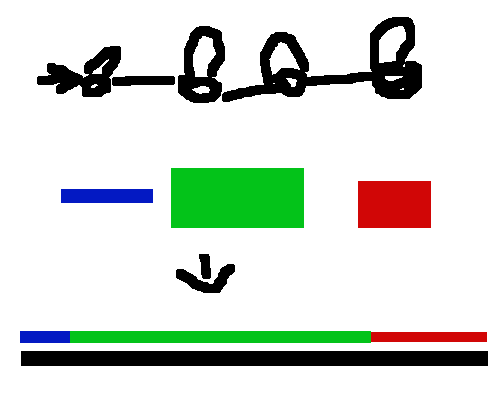
\includegraphics[scale=1.0]{images/Hmm_Chromosom_Representation.png}


\subsection*{Fitness Operator}
Die Fitness eines Chromosoms ist die durchschnittliche Log Wahrscheinlichkeit 
des Hidden Markov Models, welchen das Chromosom representiert.
Als Observations Sequenzen werden Äußerungen der Zahl 0 aus dem Free Spoken Digit Dataset verwendet

\subsection*{Mutationsoperatoren}
Mutationsoperatoren wird dies das annanas gewählt


Belegung der Parameter:

Hidden Markov Parameter 
Bei den Hidden Markov Modellen welche von den genetischen Algorithmus optimiert werden handelt es sich 
ausschließlich um Left-right Modelle mit 4 Zuständen und 128 Observationssymbolen.
Diese Werte sind relativ Arbiträr gewählt und orientieren sich an existierender Literatur zu Spracherkennung mit Hidden Markov modellen.

Als Observations-Sequenzen werden Äußerungen der Zahl 0 aus der Free Spoken Digit Database gewählt.
Welche mittels eines k-means algorithmus mit k=128 quantisiert wurden.


Genetischer Algorithmus Parameter:

Die Populationsgröße wird auf 50 beschränkt und die Anzahl der Generationen auf 100.
Das Rational für diese Entscheidung ist, dass ein Ablauf des Genetischen Algorithmus mit diesen Parametern
auf meinem Klapprechner in unter 5 minuten abläuft und 100 Generationen meißt ausreichen um den Genetischen Algorithmus konvergieren zu lassen
Die Anzahl der Observationssequenzen ist 10


\subsection*{Erweiterung des GA}
- Der genetische Algorithmus muss um einen Normalisierungsschritt erweitert werden, 
falls die Crossover oder Mutationsoperatoren keine Reihenstochastizität garantieren.
\chapter{Related Work}\label{ch:related_work}

This chapter presents the basis on which the system and later evaluation are built.
It usually contains short descriptions of previous research papers
and puts them into the context of the thesis.

\section{Code Listings}

If there is some interesting code you would like to show
in order to ease the understanding of the text,
you can just include it using the \verb+lstlisting+ environment.
Have a look at the source of this page to see how this is included:

\begin{lstlisting}[language=Go]
x := from(42);
\end{lstlisting}

You could also put the code into an external file
and include it in this document using the \verb+lstinputlisting+ command:

\lstinputlisting[language=Go,numbers=left]{listings/example.go}

Be careful not to include large files as it hampers readability.
If there is a short excerpt from a large file you would like to show,
you can also extract an explicit range of lines from it without the need to modify the source file.
This next listing only shows the conditional from the previous code:

\lstinputlisting[language=Go,numbers=left,firstline=2,lastline=5,firstnumber=2]{listings/example.go}

To use more advanced syntax highlighting
have a look at the available options of the \emph{listings} package
or use the \emph{minted} package\footnote{\url{https://texdoc.net/texmf-dist/doc/latex/minted/minted.pdf}},
which has more extensive language support and additional themes.
Both can be configured in the main file.
 % input does not start a new page
\section{Math}

In case you need to include some math,
the \emph{amsmath} package\footnote{\url{https://texdoc.net/texmf-dist/doc/latex/amsmath/amsmath.pdf}} is already included in this document.

To properly display some short formula like \( e^{i \pi} = -1\),
you can use the \verb+\( \)+ inline command.
For larger formulas, the \verb+math+ environment is more appropriate.
If you need to reference the formula multiple times,
e.g. in case it is used in theorems,
you should use the \verb+equation+ environment:

\begin{equation}
	\vec\nabla\times\vec{B}= \mu_0\vec{j}+\mu_0\varepsilon_0\frac{\partial\vec{E}}{\partial t}
	\label{func}
\end{equation}

To reference it as~\ref{func} using the \verb+\ref{}+ command,
remember to use a \verb+\label{}+.

\section{Miscellaneous}

You can use the \verb+\todo{}+ command to put obvious reminders on the side of the document.\todo{like this!}


was zum fick?

% Appendix chapters to be put here. They will be enumerated with capital letters
% if you  did not change the \documentclass options.
\appendix
% \include{content/appendix}

%Bibliography
% We strongly recommend to use bibtex to manage your bibliography. It helps you
% structure your references and helps avoiding missing important data for a correct
% quotation. If you have no other idea jabref (http://jabref.sourceforge.net/)
% might be a good idea (Java runtime environment needed).
\printbibliography

% Include the eidesstattliche Versicherung
% spellchecker:disable
%pagenumbering{null}

\

\cleardoublepage

\


\pagestyle{empty}

\selectlanguage{german}
\textbf{Eigenständigkeitserklärung}\\

Hiermit versichere ich, dass ich diese Arbeit bzw. im Fall einer Gruppenarbeit
den von mir entsprechend gekennzeichneten Anteil an der Arbeit selbständig verfasst habe.
Ich habe keine unzulässige Hilfe Dritter in Anspruch genommen. Zudem habe ich keine
anderen als die angegebenen Quellen und Hilfsmittel benutzt und alle Ausführungen
(insbesondere Zitate), die anderen Quellen wörtlich oder sinngemäß entnommen wurden,
kenntlich gemacht.
Ich versichere, dass die von mir in elektronischer Form eingereichte Version dieser Arbeit mit
den eingereichten gedruckten Exemplaren übereinstimmt.
Mir ist bekannt, dass im Falle eines Täuschungsversuches die betreffende Leistung als mit
“nicht ausreichend” (5,0) bewertet gilt. Zudem kann ein Täuschungsversuch als
Ordnungswidrigkeit mit einer Geldbuße von bis zu 50.000 Euro geahndet werden. Im Falle
eines mehrfachen oder sonstigen schwerwiegenden Täuschungsversuchs kann ich zudem
exmatrikuliert werden.
Mir ist bekannt, dass sich die Prüferin oder der Prüfer bzw. der Prüfungsausschuss zur
Feststellung der Täuschung des Einsatzes einer entsprechenden Software oder sonstiger
elektronischer Hilfsmittel bedienen kann.
\vfill
Duisburg, \today\\
$\overline{\parbox{4.8cm}{(Ort, Datum)}} ~~~~~~~~~~~~~~~~~~~~~~~~~~~ \overline{\parbox{7cm}{(Vorname Nachname)}}$


\end{document}
